\documentclass[11pt]{article}
\usepackage{longtable}
\usepackage{graphicx}
\usepackage{lineno}
%\usepackage{amssymb}
\usepackage{color}
\definecolor{darkgreen}{rgb}{0,0.5,0}
\usepackage{hyperref}
\hypersetup{colorlinks=true, urlcolor=blue, citecolor=darkgreen}
\usepackage{natbib}
\usepackage{fullpage}
\usepackage{setspace}
\usepackage{listings}
\usepackage{scrextend}
\renewcommand{\familydefault}{\sfdefault}
\def\changemargin#1#2{\list{}{\rightmargin#2\leftmargin#1}\item[]}
\let\endchangemargin=\endlist 
\begin{document}
\begin{flushleft}


{\Large
\textbf{Improving transcriptome assembly through error correction of high-throughput sequence reads}
}
\\ 
\vspace{4mm}

\noindent
Matthew D MacManes$^{1}$$^\ast$ and
Michael B. Eisen$^{1,2}$ \\
\vspace{5mm}

\bf{1} \textnormal{UC Berkeley. California Institute of Quantitative Biology, Berkeley, CA, USA} \\
\bf{2} \textnormal{Howard Hughes Medical Institute} \\
\vspace{2mm}
 
\bf{$\ast$} \textnormal{Corresponding author: \href{mailto:macmanes@gmail.com}{macmanes@gmail.com}, Twitter: \href{https://twitter.com/PeroMHC}{$@$PeroMHC}}
\end{flushleft}
\vspace{4mm}



\section*{Response to Reviewers Comments}

\hspace{5mm} Please find the attached paper, which is a revision of manuscript number 2013:04:462:0:0. The manuscript has undergone substantial change in response to comments from Titus, Mick, and Gerard (Editor).  My reading of these comments suggested several major deficits, all of which have been addressed. We know use paired-end data, compare our results using simulated data to 'real' data, and make our data publicly available. In addition to these major changes (which required that all analyses be re-worked), we also address the other concerns, including justifying our choice of methods and data types. 

The paper is much stronger as a result of this review process, and I hope you will find the changes satisfactory. \\

\noindent
Best, Matt MacManes 


\begin{enumerate}


\item The use of real versus fake data. 

\begin{addmargin}[2em]{2em}
This is an excellent suggestion. In response, I have done a parallel analysis using a random 30M PE read subset of the Trinity mouse dataset.  I choose to use 30M reads rather than the full 50M read dataset to maximize comparability, though moderate differences in coverage still exist.  \\

\noindent
With regards to analyses, the paper continues to focus mostly on the simulated data, though I now state that the results of the simulation study have been corroborated by analysis of real data.  That the finding are robust to dataset should be interpreted as evidence of general utility of these methods. 
\end{addmargin}

\item Use paired end reads.

\begin{addmargin}[2em]{2em}
I have used 30 million PE reads in this version of the paper. The results are unchanged, though the magnitude of the improvement is reduced. I believe this to be due to the general improvement of the assembly quality secondary to use of PE reads. 
\end{addmargin}

\item Deposit the data!. 
\begin{addmargin}[2em]{2em}
The data are now publicly available. The reads are available on my personal Dropbox (\url{https://www.dropbox.com/s/rkl0ihqom28smb2/empiric.reads.tar.gz} and \url{https://www.dropbox.com/s/mp8fu0tijox69ki/simulated.reads.tar.gz}). They will be moved to Dryad upon acceptance. The assemblies are available at \url{http://dx.doi.org/10.6084/m9.figshare.725715}. The code has been moved to a Github Gist \url{https://gist.github.com/macmanes}
\end{addmargin}


\item Justify the use of error correction techniques 
\begin{addmargin}[2em]{2em}
The specific error correction techniques were chosen in an attempt to cover the breadth of computational techniques, as well as to include tools commonly used, and recently benchmarked. I make this explicit in the manuscript. Of note, this version removes the program ECHO from the analysis. Given that it would have taken at least 4 weeks to run with the new PE data and empirically derived dataset, I did not have the time, given the constraints on resubmission. 
\end{addmargin}

\item Use more than just Illumina data. 
\begin{addmargin}[2em]{2em}
While I agree that expanding the paper to include different types of sequence data (454 and IonTorrent) would be interesting, it is beyond the scope of this current paper, which focuses on the current (and likely future, given the number of deployed machines) most popular sequencing technology. In addition, that each technology has a unique error model, understanding the results would not be easy, given simulated data not accessible. 
\end{addmargin}

\item What's going on with splice variants? 
\begin{addmargin}[2em]{2em}
Good question... As Titus notes in his review, the analysis of splice variants is tricky. I am quite interested in developing these methods, perhaps as part of a larger project (in connection with my work with Trinity). I think that attempting to dig into splicing here would be too much. I do note the issue in the discussion (line 230 -- ), as a potential issue with error correction. 
\end{addmargin}


\item Variable coverage and miscorrections? 
\begin{addmargin}[2em]{2em}
This is a really interesting point, and one I would have expected the developers of the various error correctors to have addressed-- They have not. I do see signs of low expressed contigs suffering from a less efficient correction (I suspect this is why Seecer did so poorly in my trials). Also, when looking at the number of corrections per read-- reads that are miscorrected tended to have more corrections than did appropriately corrected reads.
\end{addmargin}
\centerline{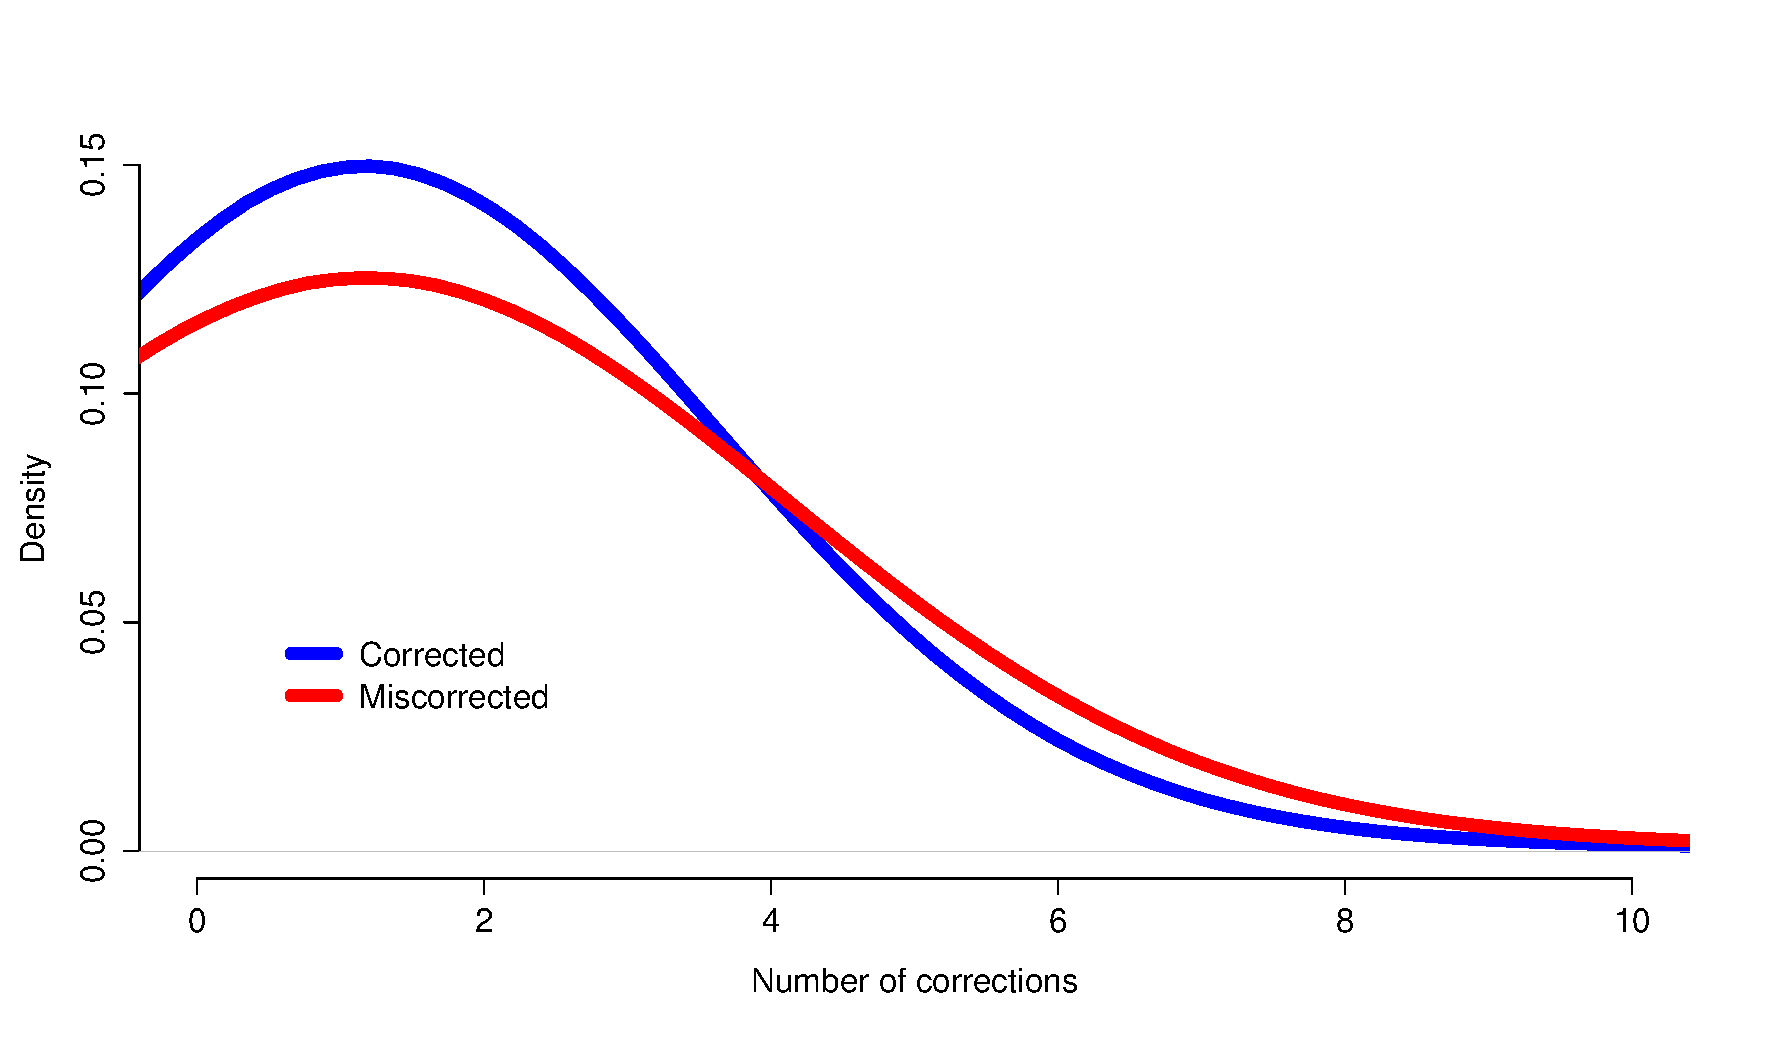
\includegraphics[width=30.0\baselineskip]{FigX.eps}}

 



\item The use of real versus fake data. 
\begin{addmargin}[2em]{2em}
\end{addmargin}






\end{enumerate}




















































\end{document}